% Shared vector grammar. Generated figure TeX files inline this source.
\documentclass[tikz,border=4mm,12pt]{standalone}
\usepackage[UTF8,fontset=fandol]{ctex}
\usepackage{amsmath,amssymb,bm}
\renewcommand{\familydefault}{\sfdefault}
\hyphenpenalty=10000
\exhyphenpenalty=10000
\usetikzlibrary{arrows.meta,backgrounds,calc}
\definecolor{Ink}{HTML}{273648}
\definecolor{Muted}{HTML}{607086}
\definecolor{Ctx}{HTML}{85898F}
\definecolor{Qst}{HTML}{4F8FA5}
\definecolor{Opt}{HTML}{5A9A6E}
\definecolor{Gen}{HTML}{B89A5E}
\definecolor{Hid}{HTML}{8A74B5}
\definecolor{Wgt}{HTML}{E0904F}
\definecolor{Lgt}{HTML}{C95B5B}
\definecolor{Idx}{HTML}{7E8B9B}
\definecolor{Msk}{HTML}{3F5A78}
\newcommand{\Unit}{0.30}
\newcommand{\Offset}{0.12}
\newcommand{\BinarySupport}{0}
\newcounter{texture}
\tikzset{
 flow/.style={-{Latex[length=2mm,width=1.5mm]},draw=Ink!75!Canvas,line width=.65pt},
 tensorlabel/.style={font=\small,text=Ink,align=center,inner sep=0pt},
 tenshape/.style={font=\scriptsize,text=Muted,align=center,inner sep=0pt},
 stage/.style={font=\small\bfseries,text=Muted,align=left,anchor=west},
 operation/.style={draw=Ink!25!Canvas,fill=Canvas,rounded corners=2pt,align=center,
  font=\small,text=Ink,inner sep=5pt,line width=.5pt},
}
% The last two axes define a matrix face. Leading axes use offset sheets.
% Every symbolic dimension maps to the same cell count throughout the set.
\newcommand{\Tensor}[9]{%
 \stepcounter{texture}
 \pgfmathsetmacro{\ww}{#5*\Unit}
 \pgfmathsetmacro{\hh}{#4*\Unit}
 \pgfmathsetmacro{\xx}{#2-\ww/2}
 \pgfmathsetmacro{\yy}{#3-\hh/2}
 \ifnum#7>0
  \foreach \s in {#7,...,1}{
   \path[draw=#6!40!Canvas,fill=Canvas,line width=.45pt,rounded corners=.7pt]
    ({\xx+\s*\Offset},{\yy+\s*\Offset}) rectangle ++(\ww,\hh);}
 \fi
 \foreach \r in {1,...,#4}{\foreach \c in {1,...,#5}{
  \ifnum\BinarySupport>0
   \pgfmathtruncatemacro{\level}{\BinarySupport==1?(\c>3-\r?75:0):(\BinarySupport==2?(\c<=4-\r?75:0):(\c<=\r?75:0))}
  \else
   \pgfmathtruncatemacro{\tone}{mod(\r*13+\c*7+\arabic{texture}*11,7)}
   \pgfmathtruncatemacro{\level}{\tone<3?30:(\tone<6?55:80)}
  \fi
  \path[fill=#6!\level!Canvas,rounded corners=.5pt]
   ({\xx+(\c-1)*\Unit+.021},{\yy+\hh-\r*\Unit+.021})
    rectangle ++({\Unit-.042},{\Unit-.042});}}
 \ifnum\BinarySupport>0
  \path[draw=Msk!35!Canvas,line width=.4pt] (\xx,\yy) rectangle ++(\ww,\hh);
 \fi
 \coordinate (#1-w) at (\xx,#3);
 \coordinate (#1-e) at ({\xx+\ww+#7*\Offset},#3);
 \node[tensorlabel] at (#2,{\yy-.28}) {$#8$};
 \node[tenshape] at (#2,{\yy-.63}) {$#9$};
}
% Exact binary support; row i is a query and column j a key.
\newcommand{\Support}[5]{%
 \foreach \i in {1,...,#4}{\foreach \j in {1,...,#4}{
  \pgfmathtruncatemacro{\on}{#5}
  \ifnum\on>0
   \path[fill=Msk!65!Canvas,rounded corners=.4pt]
    ({#2+(\j-1)*\Unit+.021},{#3-\i*\Unit+.021})
     rectangle ++({\Unit-.042},{\Unit-.042});
  \fi}}
 \path[draw=Ink!35!Canvas,line width=.4pt] (#2,#3) rectangle ++({#4*\Unit},{-#4*\Unit});
}
\newcommand{\Meaning}[7]{%
 \node[anchor=north west,fill=Ink!4!Canvas,rounded corners=3pt,inner sep=9pt,
  text width=#3cm-18pt,align=left,font=\small] (meaning) at (#1,#2) {
  \begin{tabular}{@{}p{1.8cm}@{\hspace{7pt}}p{\dimexpr #3cm-2.8cm\relax}@{}}
   \textbf{#4} & \raggedright #5\tabularnewline[6pt]
   \textbf{#6} & \raggedright #7\tabularnewline
  \end{tabular}};
}

\definecolor{Canvas}{HTML}{18212C}
\definecolor{Ink}{HTML}{E2EAF3}
\definecolor{Muted}{HTML}{AABCD0}
\definecolor{Ctx}{HTML}{ABB3BE}
\definecolor{Qst}{HTML}{72B8D0}
\definecolor{Opt}{HTML}{83C396}
\definecolor{Gen}{HTML}{D9BC7B}
\definecolor{Hid}{HTML}{B49BDB}
\definecolor{Wgt}{HTML}{F0AB71}
\definecolor{Lgt}{HTML}{ED9191}
\definecolor{Idx}{HTML}{A9BBD1}
\definecolor{Msk}{HTML}{91B6DF}
\pagecolor{Canvas}

\providecolor{Canvas}{HTML}{FFFFFF}
\begin{document}
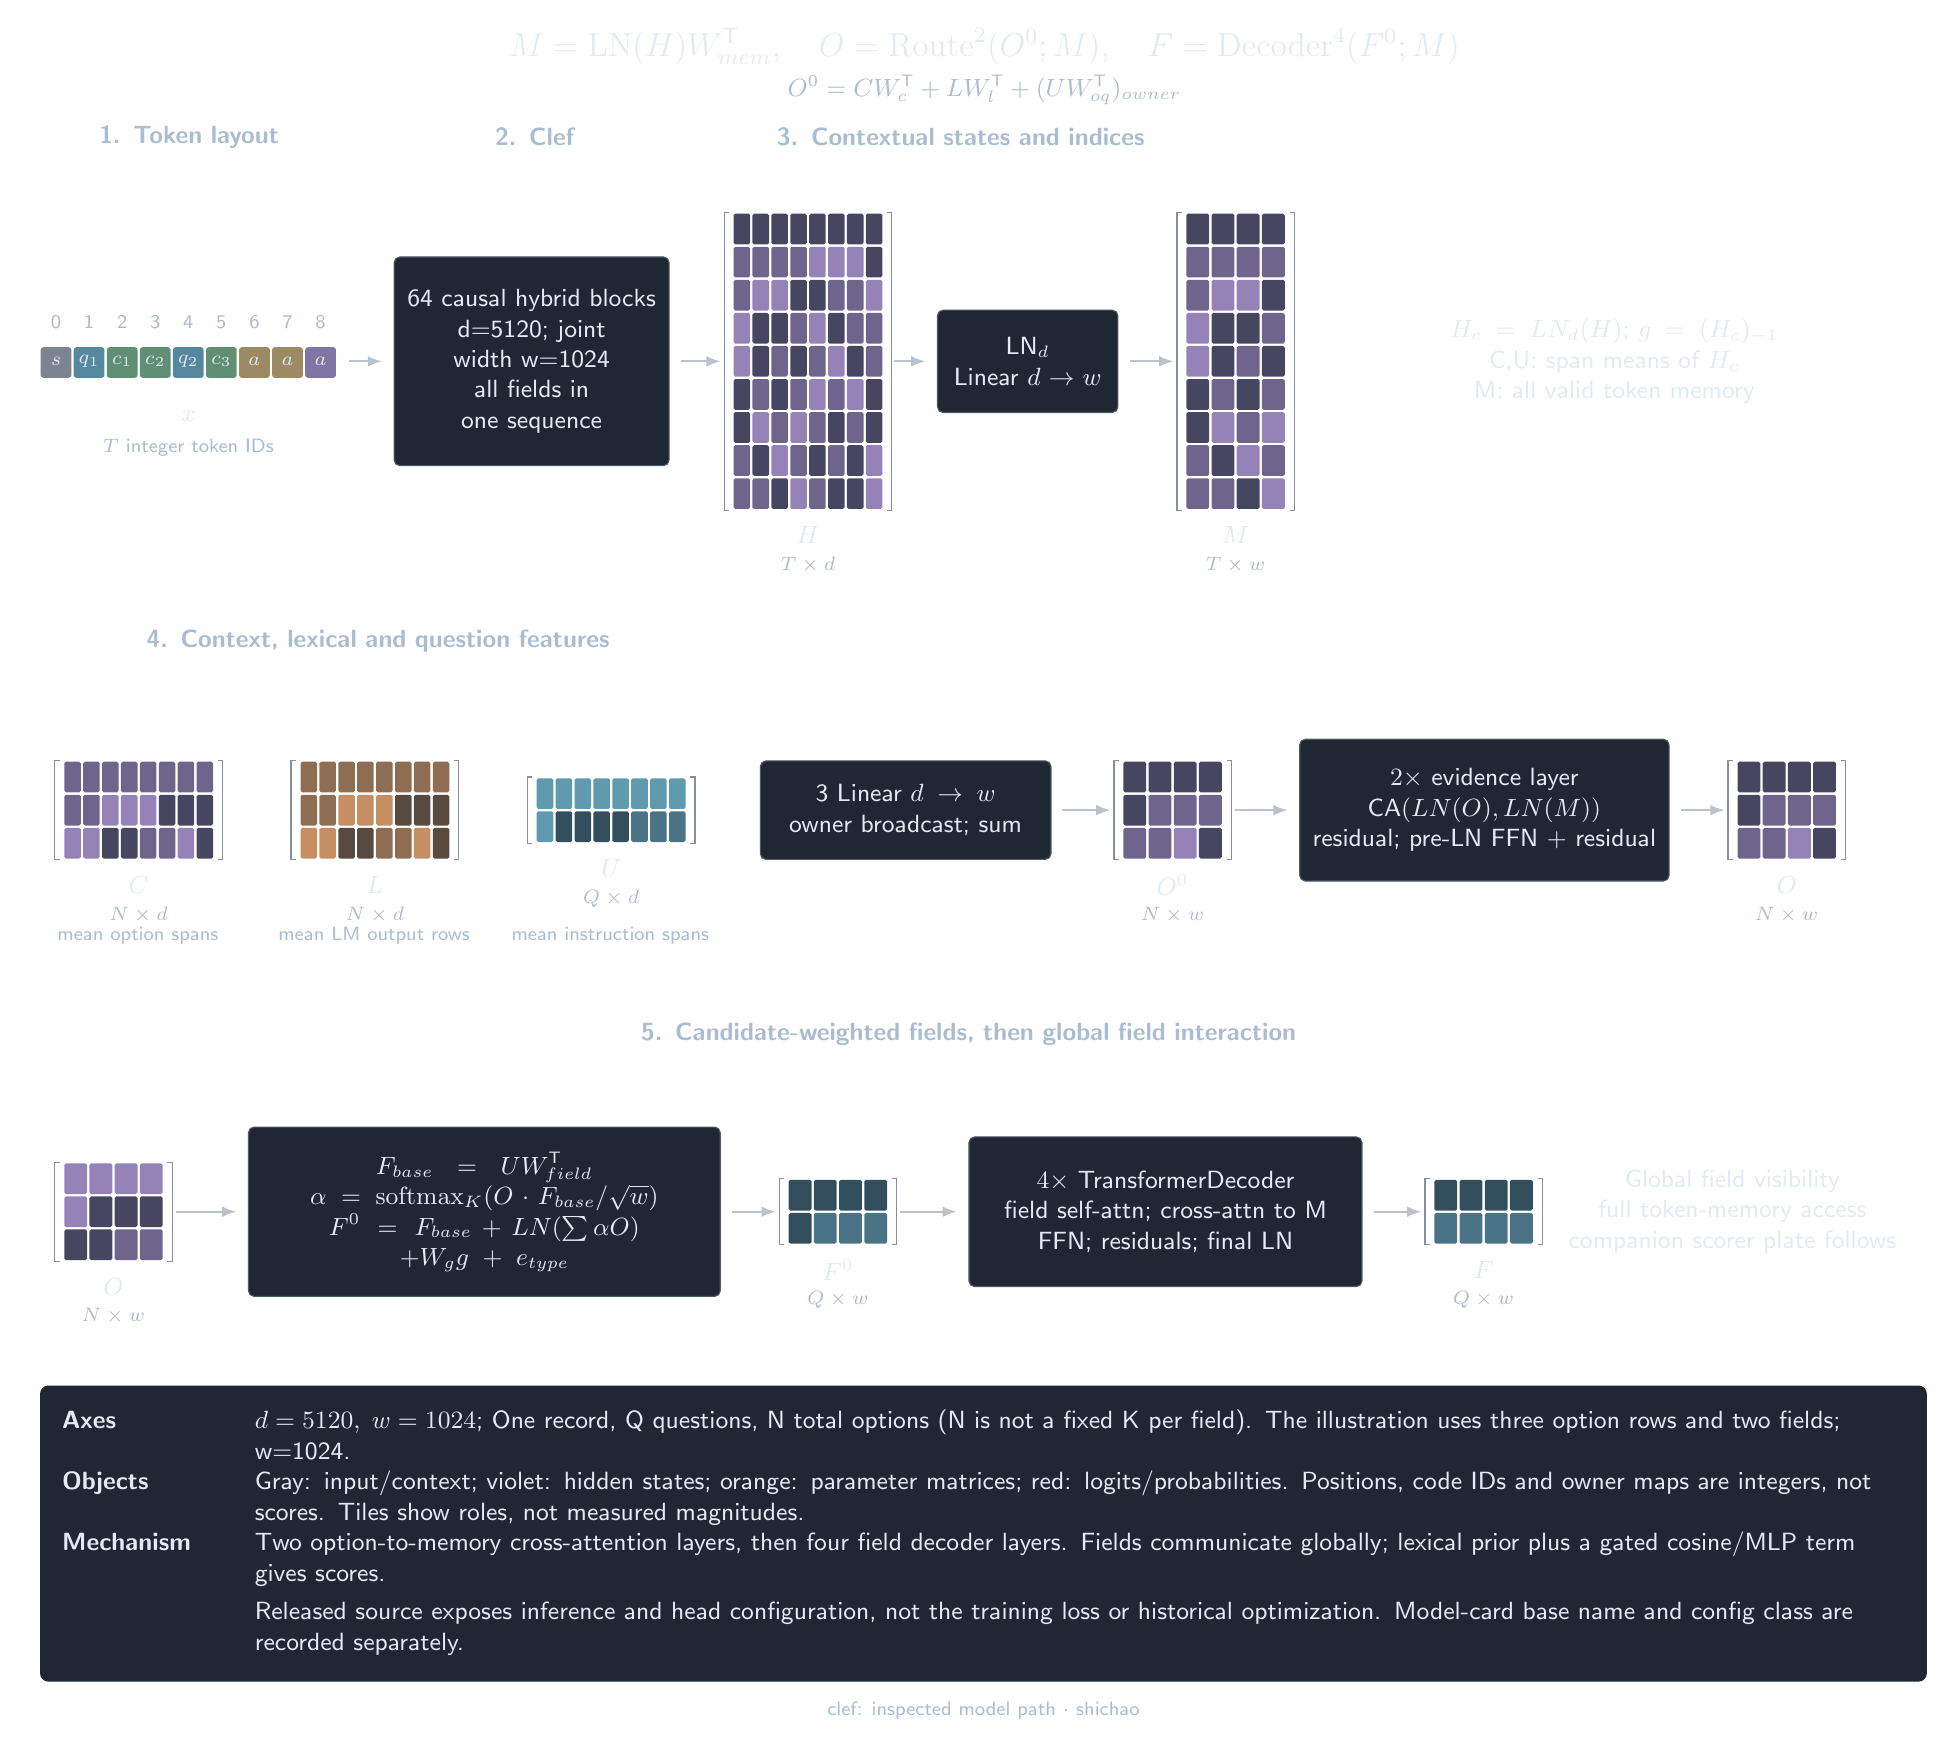
\begin{tikzpicture}[x=1cm,y=1cm,text=Ink]
\node[font=\large,text=Ink,anchor=center,align=center,inner sep=0pt] at (12.000,4.000) {$\displaystyle M=\operatorname{LN}(H)W_{mem}^{\mathsf T},\quad O=\operatorname{Route}^{2}(O^0;M),\quad F=\operatorname{Decoder}^{4}(F^0;M)$};
\node[font=\small,text=Muted,anchor=center,align=center,inner sep=0pt,text width=4.1cm] at (1.900,2.850) {\textbf{1. Token layout}};
\node[font=\small,text=Muted,anchor=center,align=center,inner sep=0pt,text width=3.6cm] at (6.300,2.850) {\textbf{2. Clef}};
\node[font=\small,text=Muted,anchor=center,align=center,inner sep=0pt,text width=5.6cm] at (11.700,2.850) {\textbf{3. Contextual states and indices}};
\path[fill=Ctx!68!Canvas,rounded corners=1pt] (0.015,-0.210) rectangle ++(0.390,0.390);
\node[font=\scriptsize,text=Ink,anchor=center,align=center,inner sep=0pt] at (0.210,0.000) {$s$};
\node[font=\scriptsize,text=Muted,anchor=center,align=center,inner sep=0pt] at (0.210,0.500) {0};
\path[fill=Qst!68!Canvas,rounded corners=1pt] (0.435,-0.210) rectangle ++(0.390,0.390);
\node[font=\scriptsize,text=Ink,anchor=center,align=center,inner sep=0pt] at (0.630,0.000) {$q_1$};
\node[font=\scriptsize,text=Muted,anchor=center,align=center,inner sep=0pt] at (0.630,0.500) {1};
\path[fill=Opt!68!Canvas,rounded corners=1pt] (0.855,-0.210) rectangle ++(0.390,0.390);
\node[font=\scriptsize,text=Ink,anchor=center,align=center,inner sep=0pt] at (1.050,0.000) {$c_1$};
\node[font=\scriptsize,text=Muted,anchor=center,align=center,inner sep=0pt] at (1.050,0.500) {2};
\path[fill=Opt!68!Canvas,rounded corners=1pt] (1.275,-0.210) rectangle ++(0.390,0.390);
\node[font=\scriptsize,text=Ink,anchor=center,align=center,inner sep=0pt] at (1.470,0.000) {$c_2$};
\node[font=\scriptsize,text=Muted,anchor=center,align=center,inner sep=0pt] at (1.470,0.500) {3};
\path[fill=Qst!68!Canvas,rounded corners=1pt] (1.695,-0.210) rectangle ++(0.390,0.390);
\node[font=\scriptsize,text=Ink,anchor=center,align=center,inner sep=0pt] at (1.890,0.000) {$q_2$};
\node[font=\scriptsize,text=Muted,anchor=center,align=center,inner sep=0pt] at (1.890,0.500) {4};
\path[fill=Opt!68!Canvas,rounded corners=1pt] (2.115,-0.210) rectangle ++(0.390,0.390);
\node[font=\scriptsize,text=Ink,anchor=center,align=center,inner sep=0pt] at (2.310,0.000) {$c_3$};
\node[font=\scriptsize,text=Muted,anchor=center,align=center,inner sep=0pt] at (2.310,0.500) {5};
\path[fill=Gen!68!Canvas,rounded corners=1pt] (2.535,-0.210) rectangle ++(0.390,0.390);
\node[font=\scriptsize,text=Ink,anchor=center,align=center,inner sep=0pt] at (2.730,0.000) {$a$};
\node[font=\scriptsize,text=Muted,anchor=center,align=center,inner sep=0pt] at (2.730,0.500) {6};
\path[fill=Gen!68!Canvas,rounded corners=1pt] (2.955,-0.210) rectangle ++(0.390,0.390);
\node[font=\scriptsize,text=Ink,anchor=center,align=center,inner sep=0pt] at (3.150,0.000) {$a$};
\node[font=\scriptsize,text=Muted,anchor=center,align=center,inner sep=0pt] at (3.150,0.500) {7};
\path[fill=Hid!68!Canvas,rounded corners=1pt] (3.375,-0.210) rectangle ++(0.390,0.390);
\node[font=\scriptsize,text=Ink,anchor=center,align=center,inner sep=0pt] at (3.570,0.000) {$a$};
\node[font=\scriptsize,text=Muted,anchor=center,align=center,inner sep=0pt] at (3.570,0.500) {8};
\node[font=\small,text=Ink,anchor=center,align=center,inner sep=0pt] at (1.890,-0.700) {$x$};
\node[font=\scriptsize,text=Muted,anchor=center,align=center,inner sep=0pt] at (1.890,-1.100) {$T$ integer token IDs};
\node[draw=Ink!28!Canvas,fill=Ink!3!Canvas,rounded corners=2pt,font=\small,text width=3.280cm,align=center,inner sep=3pt,minimum height=2.650cm] at (6.250,0.000) {64 causal hybrid blocks\\d=5120; joint width w=1024\\all fields in one sequence};
\path[fill=Hid!30!Canvas,rounded corners=.6pt] (8.815,1.485) rectangle ++(0.210,0.390);
\path[fill=Hid!30!Canvas,rounded corners=.6pt] (9.055,1.485) rectangle ++(0.210,0.390);
\path[fill=Hid!30!Canvas,rounded corners=.6pt] (9.295,1.485) rectangle ++(0.210,0.390);
\path[fill=Hid!30!Canvas,rounded corners=.6pt] (9.535,1.485) rectangle ++(0.210,0.390);
\path[fill=Hid!30!Canvas,rounded corners=.6pt] (9.775,1.485) rectangle ++(0.210,0.390);
\path[fill=Hid!30!Canvas,rounded corners=.6pt] (10.015,1.485) rectangle ++(0.210,0.390);
\path[fill=Hid!30!Canvas,rounded corners=.6pt] (10.255,1.485) rectangle ++(0.210,0.390);
\path[fill=Hid!30!Canvas,rounded corners=.6pt] (10.495,1.485) rectangle ++(0.210,0.390);
\path[fill=Hid!55!Canvas,rounded corners=.6pt] (8.815,1.065) rectangle ++(0.210,0.390);
\path[fill=Hid!55!Canvas,rounded corners=.6pt] (9.055,1.065) rectangle ++(0.210,0.390);
\path[fill=Hid!55!Canvas,rounded corners=.6pt] (9.295,1.065) rectangle ++(0.210,0.390);
\path[fill=Hid!55!Canvas,rounded corners=.6pt] (9.535,1.065) rectangle ++(0.210,0.390);
\path[fill=Hid!80!Canvas,rounded corners=.6pt] (9.775,1.065) rectangle ++(0.210,0.390);
\path[fill=Hid!80!Canvas,rounded corners=.6pt] (10.015,1.065) rectangle ++(0.210,0.390);
\path[fill=Hid!80!Canvas,rounded corners=.6pt] (10.255,1.065) rectangle ++(0.210,0.390);
\path[fill=Hid!30!Canvas,rounded corners=.6pt] (10.495,1.065) rectangle ++(0.210,0.390);
\path[fill=Hid!55!Canvas,rounded corners=.6pt] (8.815,0.645) rectangle ++(0.210,0.390);
\path[fill=Hid!80!Canvas,rounded corners=.6pt] (9.055,0.645) rectangle ++(0.210,0.390);
\path[fill=Hid!80!Canvas,rounded corners=.6pt] (9.295,0.645) rectangle ++(0.210,0.390);
\path[fill=Hid!30!Canvas,rounded corners=.6pt] (9.535,0.645) rectangle ++(0.210,0.390);
\path[fill=Hid!30!Canvas,rounded corners=.6pt] (9.775,0.645) rectangle ++(0.210,0.390);
\path[fill=Hid!55!Canvas,rounded corners=.6pt] (10.015,0.645) rectangle ++(0.210,0.390);
\path[fill=Hid!55!Canvas,rounded corners=.6pt] (10.255,0.645) rectangle ++(0.210,0.390);
\path[fill=Hid!80!Canvas,rounded corners=.6pt] (10.495,0.645) rectangle ++(0.210,0.390);
\path[fill=Hid!80!Canvas,rounded corners=.6pt] (8.815,0.225) rectangle ++(0.210,0.390);
\path[fill=Hid!30!Canvas,rounded corners=.6pt] (9.055,0.225) rectangle ++(0.210,0.390);
\path[fill=Hid!30!Canvas,rounded corners=.6pt] (9.295,0.225) rectangle ++(0.210,0.390);
\path[fill=Hid!55!Canvas,rounded corners=.6pt] (9.535,0.225) rectangle ++(0.210,0.390);
\path[fill=Hid!80!Canvas,rounded corners=.6pt] (9.775,0.225) rectangle ++(0.210,0.390);
\path[fill=Hid!30!Canvas,rounded corners=.6pt] (10.015,0.225) rectangle ++(0.210,0.390);
\path[fill=Hid!55!Canvas,rounded corners=.6pt] (10.255,0.225) rectangle ++(0.210,0.390);
\path[fill=Hid!55!Canvas,rounded corners=.6pt] (10.495,0.225) rectangle ++(0.210,0.390);
\path[fill=Hid!80!Canvas,rounded corners=.6pt] (8.815,-0.195) rectangle ++(0.210,0.390);
\path[fill=Hid!30!Canvas,rounded corners=.6pt] (9.055,-0.195) rectangle ++(0.210,0.390);
\path[fill=Hid!55!Canvas,rounded corners=.6pt] (9.295,-0.195) rectangle ++(0.210,0.390);
\path[fill=Hid!30!Canvas,rounded corners=.6pt] (9.535,-0.195) rectangle ++(0.210,0.390);
\path[fill=Hid!55!Canvas,rounded corners=.6pt] (9.775,-0.195) rectangle ++(0.210,0.390);
\path[fill=Hid!80!Canvas,rounded corners=.6pt] (10.015,-0.195) rectangle ++(0.210,0.390);
\path[fill=Hid!30!Canvas,rounded corners=.6pt] (10.255,-0.195) rectangle ++(0.210,0.390);
\path[fill=Hid!55!Canvas,rounded corners=.6pt] (10.495,-0.195) rectangle ++(0.210,0.390);
\path[fill=Hid!30!Canvas,rounded corners=.6pt] (8.815,-0.615) rectangle ++(0.210,0.390);
\path[fill=Hid!55!Canvas,rounded corners=.6pt] (9.055,-0.615) rectangle ++(0.210,0.390);
\path[fill=Hid!30!Canvas,rounded corners=.6pt] (9.295,-0.615) rectangle ++(0.210,0.390);
\path[fill=Hid!55!Canvas,rounded corners=.6pt] (9.535,-0.615) rectangle ++(0.210,0.390);
\path[fill=Hid!80!Canvas,rounded corners=.6pt] (9.775,-0.615) rectangle ++(0.210,0.390);
\path[fill=Hid!55!Canvas,rounded corners=.6pt] (10.015,-0.615) rectangle ++(0.210,0.390);
\path[fill=Hid!80!Canvas,rounded corners=.6pt] (10.255,-0.615) rectangle ++(0.210,0.390);
\path[fill=Hid!30!Canvas,rounded corners=.6pt] (10.495,-0.615) rectangle ++(0.210,0.390);
\path[fill=Hid!30!Canvas,rounded corners=.6pt] (8.815,-1.035) rectangle ++(0.210,0.390);
\path[fill=Hid!80!Canvas,rounded corners=.6pt] (9.055,-1.035) rectangle ++(0.210,0.390);
\path[fill=Hid!55!Canvas,rounded corners=.6pt] (9.295,-1.035) rectangle ++(0.210,0.390);
\path[fill=Hid!80!Canvas,rounded corners=.6pt] (9.535,-1.035) rectangle ++(0.210,0.390);
\path[fill=Hid!55!Canvas,rounded corners=.6pt] (9.775,-1.035) rectangle ++(0.210,0.390);
\path[fill=Hid!30!Canvas,rounded corners=.6pt] (10.015,-1.035) rectangle ++(0.210,0.390);
\path[fill=Hid!55!Canvas,rounded corners=.6pt] (10.255,-1.035) rectangle ++(0.210,0.390);
\path[fill=Hid!30!Canvas,rounded corners=.6pt] (10.495,-1.035) rectangle ++(0.210,0.390);
\path[fill=Hid!55!Canvas,rounded corners=.6pt] (8.815,-1.455) rectangle ++(0.210,0.390);
\path[fill=Hid!30!Canvas,rounded corners=.6pt] (9.055,-1.455) rectangle ++(0.210,0.390);
\path[fill=Hid!80!Canvas,rounded corners=.6pt] (9.295,-1.455) rectangle ++(0.210,0.390);
\path[fill=Hid!55!Canvas,rounded corners=.6pt] (9.535,-1.455) rectangle ++(0.210,0.390);
\path[fill=Hid!30!Canvas,rounded corners=.6pt] (9.775,-1.455) rectangle ++(0.210,0.390);
\path[fill=Hid!55!Canvas,rounded corners=.6pt] (10.015,-1.455) rectangle ++(0.210,0.390);
\path[fill=Hid!30!Canvas,rounded corners=.6pt] (10.255,-1.455) rectangle ++(0.210,0.390);
\path[fill=Hid!80!Canvas,rounded corners=.6pt] (10.495,-1.455) rectangle ++(0.210,0.390);
\path[fill=Hid!55!Canvas,rounded corners=.6pt] (8.815,-1.875) rectangle ++(0.210,0.390);
\path[fill=Hid!55!Canvas,rounded corners=.6pt] (9.055,-1.875) rectangle ++(0.210,0.390);
\path[fill=Hid!30!Canvas,rounded corners=.6pt] (9.295,-1.875) rectangle ++(0.210,0.390);
\path[fill=Hid!80!Canvas,rounded corners=.6pt] (9.535,-1.875) rectangle ++(0.210,0.390);
\path[fill=Hid!55!Canvas,rounded corners=.6pt] (9.775,-1.875) rectangle ++(0.210,0.390);
\path[fill=Hid!30!Canvas,rounded corners=.6pt] (10.015,-1.875) rectangle ++(0.210,0.390);
\path[fill=Hid!30!Canvas,rounded corners=.6pt] (10.255,-1.875) rectangle ++(0.210,0.390);
\path[fill=Hid!80!Canvas,rounded corners=.6pt] (10.495,-1.875) rectangle ++(0.210,0.390);
\draw[draw=Ink!55!Canvas,line width=.45pt] (8.755,1.890) -- ++(-.06,0) -- ++(0,-3.780) -- ++(.06,0);
\draw[draw=Ink!55!Canvas,line width=.45pt] (10.765,1.890) -- ++(.06,0) -- ++(0,-3.780) -- ++(-.06,0);
\node[font=\small,text=Ink,anchor=center,align=center,inner sep=0pt] at (9.760,-2.210) {$H$};
\node[font=\scriptsize,text=Muted,anchor=center,align=center,inner sep=0pt] at (9.760,-2.590) {$T\times d$};
\begin{scope}[on background layer]
\draw[-{Latex[length=1.8mm]},draw=Ink!80!Canvas,line width=.7pt] (3.930,0.000) -- (4.350,0.000);
\end{scope}
\begin{scope}[on background layer]
\draw[-{Latex[length=1.8mm]},draw=Ink!80!Canvas,line width=.7pt] (8.150,0.000) -- (8.650,0.000);
\end{scope}
\node[font=\small,text=Muted,anchor=center,align=center,inner sep=0pt] at (12.000,3.450) {$O^0=CW_c^{\mathsf T}+LW_l^{\mathsf T}+(UW_{oq}^{\mathsf T})_{owner}$};
\node[draw=Ink!28!Canvas,fill=Ink!3!Canvas,rounded corners=2pt,font=\small,text width=2.080cm,align=center,inner sep=3pt,minimum height=1.300cm] at (12.550,0.000) {LN$_d$\\Linear $d\to w$};
\begin{scope}[on background layer]
\draw[-{Latex[length=1.8mm]},draw=Ink!80!Canvas,line width=.7pt] (10.850,0.000) -- (11.250,0.000);
\end{scope}
\begin{scope}[on background layer]
\draw[-{Latex[length=1.8mm]},draw=Ink!80!Canvas,line width=.7pt] (13.850,0.000) -- (14.400,0.000);
\end{scope}
\path[fill=Hid!30!Canvas,rounded corners=.6pt] (14.565,1.485) rectangle ++(0.290,0.390);
\path[fill=Hid!30!Canvas,rounded corners=.6pt] (14.885,1.485) rectangle ++(0.290,0.390);
\path[fill=Hid!30!Canvas,rounded corners=.6pt] (15.205,1.485) rectangle ++(0.290,0.390);
\path[fill=Hid!30!Canvas,rounded corners=.6pt] (15.525,1.485) rectangle ++(0.290,0.390);
\path[fill=Hid!55!Canvas,rounded corners=.6pt] (14.565,1.065) rectangle ++(0.290,0.390);
\path[fill=Hid!55!Canvas,rounded corners=.6pt] (14.885,1.065) rectangle ++(0.290,0.390);
\path[fill=Hid!55!Canvas,rounded corners=.6pt] (15.205,1.065) rectangle ++(0.290,0.390);
\path[fill=Hid!55!Canvas,rounded corners=.6pt] (15.525,1.065) rectangle ++(0.290,0.390);
\path[fill=Hid!55!Canvas,rounded corners=.6pt] (14.565,0.645) rectangle ++(0.290,0.390);
\path[fill=Hid!80!Canvas,rounded corners=.6pt] (14.885,0.645) rectangle ++(0.290,0.390);
\path[fill=Hid!80!Canvas,rounded corners=.6pt] (15.205,0.645) rectangle ++(0.290,0.390);
\path[fill=Hid!30!Canvas,rounded corners=.6pt] (15.525,0.645) rectangle ++(0.290,0.390);
\path[fill=Hid!80!Canvas,rounded corners=.6pt] (14.565,0.225) rectangle ++(0.290,0.390);
\path[fill=Hid!30!Canvas,rounded corners=.6pt] (14.885,0.225) rectangle ++(0.290,0.390);
\path[fill=Hid!30!Canvas,rounded corners=.6pt] (15.205,0.225) rectangle ++(0.290,0.390);
\path[fill=Hid!55!Canvas,rounded corners=.6pt] (15.525,0.225) rectangle ++(0.290,0.390);
\path[fill=Hid!80!Canvas,rounded corners=.6pt] (14.565,-0.195) rectangle ++(0.290,0.390);
\path[fill=Hid!30!Canvas,rounded corners=.6pt] (14.885,-0.195) rectangle ++(0.290,0.390);
\path[fill=Hid!55!Canvas,rounded corners=.6pt] (15.205,-0.195) rectangle ++(0.290,0.390);
\path[fill=Hid!30!Canvas,rounded corners=.6pt] (15.525,-0.195) rectangle ++(0.290,0.390);
\path[fill=Hid!30!Canvas,rounded corners=.6pt] (14.565,-0.615) rectangle ++(0.290,0.390);
\path[fill=Hid!55!Canvas,rounded corners=.6pt] (14.885,-0.615) rectangle ++(0.290,0.390);
\path[fill=Hid!30!Canvas,rounded corners=.6pt] (15.205,-0.615) rectangle ++(0.290,0.390);
\path[fill=Hid!55!Canvas,rounded corners=.6pt] (15.525,-0.615) rectangle ++(0.290,0.390);
\path[fill=Hid!30!Canvas,rounded corners=.6pt] (14.565,-1.035) rectangle ++(0.290,0.390);
\path[fill=Hid!80!Canvas,rounded corners=.6pt] (14.885,-1.035) rectangle ++(0.290,0.390);
\path[fill=Hid!55!Canvas,rounded corners=.6pt] (15.205,-1.035) rectangle ++(0.290,0.390);
\path[fill=Hid!80!Canvas,rounded corners=.6pt] (15.525,-1.035) rectangle ++(0.290,0.390);
\path[fill=Hid!55!Canvas,rounded corners=.6pt] (14.565,-1.455) rectangle ++(0.290,0.390);
\path[fill=Hid!30!Canvas,rounded corners=.6pt] (14.885,-1.455) rectangle ++(0.290,0.390);
\path[fill=Hid!80!Canvas,rounded corners=.6pt] (15.205,-1.455) rectangle ++(0.290,0.390);
\path[fill=Hid!55!Canvas,rounded corners=.6pt] (15.525,-1.455) rectangle ++(0.290,0.390);
\path[fill=Hid!55!Canvas,rounded corners=.6pt] (14.565,-1.875) rectangle ++(0.290,0.390);
\path[fill=Hid!55!Canvas,rounded corners=.6pt] (14.885,-1.875) rectangle ++(0.290,0.390);
\path[fill=Hid!30!Canvas,rounded corners=.6pt] (15.205,-1.875) rectangle ++(0.290,0.390);
\path[fill=Hid!80!Canvas,rounded corners=.6pt] (15.525,-1.875) rectangle ++(0.290,0.390);
\draw[draw=Ink!55!Canvas,line width=.45pt] (14.505,1.890) -- ++(-.06,0) -- ++(0,-3.780) -- ++(.06,0);
\draw[draw=Ink!55!Canvas,line width=.45pt] (15.875,1.890) -- ++(.06,0) -- ++(0,-3.780) -- ++(-.06,0);
\node[font=\small,text=Ink,anchor=center,align=center,inner sep=0pt] at (15.190,-2.210) {$M$};
\node[font=\scriptsize,text=Muted,anchor=center,align=center,inner sep=0pt] at (15.190,-2.590) {$T\times w$};
\node[font=\small,text=Ink,anchor=center,align=center,inner sep=0pt,text width=5.4cm] at (20.000,0.000) {$H_c=LN_d(H)$; $g=(H_c)_{-1}$\\C,U: span means of $H_c$\\M: all valid token memory};
\node[font=\small,text=Muted,anchor=center,align=center,inner sep=0pt,text width=8.8cm] at (4.300,-3.550) {\textbf{4. Context, lexical and question features}};
\path[fill=Hid!55!Canvas,rounded corners=.6pt] (0.315,-5.475) rectangle ++(0.210,0.390);
\path[fill=Hid!55!Canvas,rounded corners=.6pt] (0.555,-5.475) rectangle ++(0.210,0.390);
\path[fill=Hid!55!Canvas,rounded corners=.6pt] (0.795,-5.475) rectangle ++(0.210,0.390);
\path[fill=Hid!55!Canvas,rounded corners=.6pt] (1.035,-5.475) rectangle ++(0.210,0.390);
\path[fill=Hid!55!Canvas,rounded corners=.6pt] (1.275,-5.475) rectangle ++(0.210,0.390);
\path[fill=Hid!55!Canvas,rounded corners=.6pt] (1.515,-5.475) rectangle ++(0.210,0.390);
\path[fill=Hid!55!Canvas,rounded corners=.6pt] (1.755,-5.475) rectangle ++(0.210,0.390);
\path[fill=Hid!55!Canvas,rounded corners=.6pt] (1.995,-5.475) rectangle ++(0.210,0.390);
\path[fill=Hid!55!Canvas,rounded corners=.6pt] (0.315,-5.895) rectangle ++(0.210,0.390);
\path[fill=Hid!55!Canvas,rounded corners=.6pt] (0.555,-5.895) rectangle ++(0.210,0.390);
\path[fill=Hid!80!Canvas,rounded corners=.6pt] (0.795,-5.895) rectangle ++(0.210,0.390);
\path[fill=Hid!80!Canvas,rounded corners=.6pt] (1.035,-5.895) rectangle ++(0.210,0.390);
\path[fill=Hid!80!Canvas,rounded corners=.6pt] (1.275,-5.895) rectangle ++(0.210,0.390);
\path[fill=Hid!30!Canvas,rounded corners=.6pt] (1.515,-5.895) rectangle ++(0.210,0.390);
\path[fill=Hid!30!Canvas,rounded corners=.6pt] (1.755,-5.895) rectangle ++(0.210,0.390);
\path[fill=Hid!30!Canvas,rounded corners=.6pt] (1.995,-5.895) rectangle ++(0.210,0.390);
\path[fill=Hid!80!Canvas,rounded corners=.6pt] (0.315,-6.315) rectangle ++(0.210,0.390);
\path[fill=Hid!80!Canvas,rounded corners=.6pt] (0.555,-6.315) rectangle ++(0.210,0.390);
\path[fill=Hid!30!Canvas,rounded corners=.6pt] (0.795,-6.315) rectangle ++(0.210,0.390);
\path[fill=Hid!30!Canvas,rounded corners=.6pt] (1.035,-6.315) rectangle ++(0.210,0.390);
\path[fill=Hid!55!Canvas,rounded corners=.6pt] (1.275,-6.315) rectangle ++(0.210,0.390);
\path[fill=Hid!55!Canvas,rounded corners=.6pt] (1.515,-6.315) rectangle ++(0.210,0.390);
\path[fill=Hid!80!Canvas,rounded corners=.6pt] (1.755,-6.315) rectangle ++(0.210,0.390);
\path[fill=Hid!30!Canvas,rounded corners=.6pt] (1.995,-6.315) rectangle ++(0.210,0.390);
\draw[draw=Ink!55!Canvas,line width=.45pt] (0.255,-5.070) -- ++(-.06,0) -- ++(0,-1.260) -- ++(.06,0);
\draw[draw=Ink!55!Canvas,line width=.45pt] (2.265,-5.070) -- ++(.06,0) -- ++(0,-1.260) -- ++(-.06,0);
\node[font=\small,text=Ink,anchor=center,align=center,inner sep=0pt] at (1.260,-6.650) {$C$};
\node[font=\scriptsize,text=Muted,anchor=center,align=center,inner sep=0pt] at (1.260,-7.030) {$N\times d$};
\path[fill=Wgt!55!Canvas,rounded corners=.6pt] (3.315,-5.475) rectangle ++(0.210,0.390);
\path[fill=Wgt!55!Canvas,rounded corners=.6pt] (3.555,-5.475) rectangle ++(0.210,0.390);
\path[fill=Wgt!55!Canvas,rounded corners=.6pt] (3.795,-5.475) rectangle ++(0.210,0.390);
\path[fill=Wgt!55!Canvas,rounded corners=.6pt] (4.035,-5.475) rectangle ++(0.210,0.390);
\path[fill=Wgt!55!Canvas,rounded corners=.6pt] (4.275,-5.475) rectangle ++(0.210,0.390);
\path[fill=Wgt!55!Canvas,rounded corners=.6pt] (4.515,-5.475) rectangle ++(0.210,0.390);
\path[fill=Wgt!55!Canvas,rounded corners=.6pt] (4.755,-5.475) rectangle ++(0.210,0.390);
\path[fill=Wgt!55!Canvas,rounded corners=.6pt] (4.995,-5.475) rectangle ++(0.210,0.390);
\path[fill=Wgt!55!Canvas,rounded corners=.6pt] (3.315,-5.895) rectangle ++(0.210,0.390);
\path[fill=Wgt!55!Canvas,rounded corners=.6pt] (3.555,-5.895) rectangle ++(0.210,0.390);
\path[fill=Wgt!80!Canvas,rounded corners=.6pt] (3.795,-5.895) rectangle ++(0.210,0.390);
\path[fill=Wgt!80!Canvas,rounded corners=.6pt] (4.035,-5.895) rectangle ++(0.210,0.390);
\path[fill=Wgt!80!Canvas,rounded corners=.6pt] (4.275,-5.895) rectangle ++(0.210,0.390);
\path[fill=Wgt!30!Canvas,rounded corners=.6pt] (4.515,-5.895) rectangle ++(0.210,0.390);
\path[fill=Wgt!30!Canvas,rounded corners=.6pt] (4.755,-5.895) rectangle ++(0.210,0.390);
\path[fill=Wgt!30!Canvas,rounded corners=.6pt] (4.995,-5.895) rectangle ++(0.210,0.390);
\path[fill=Wgt!80!Canvas,rounded corners=.6pt] (3.315,-6.315) rectangle ++(0.210,0.390);
\path[fill=Wgt!80!Canvas,rounded corners=.6pt] (3.555,-6.315) rectangle ++(0.210,0.390);
\path[fill=Wgt!30!Canvas,rounded corners=.6pt] (3.795,-6.315) rectangle ++(0.210,0.390);
\path[fill=Wgt!30!Canvas,rounded corners=.6pt] (4.035,-6.315) rectangle ++(0.210,0.390);
\path[fill=Wgt!55!Canvas,rounded corners=.6pt] (4.275,-6.315) rectangle ++(0.210,0.390);
\path[fill=Wgt!55!Canvas,rounded corners=.6pt] (4.515,-6.315) rectangle ++(0.210,0.390);
\path[fill=Wgt!80!Canvas,rounded corners=.6pt] (4.755,-6.315) rectangle ++(0.210,0.390);
\path[fill=Wgt!30!Canvas,rounded corners=.6pt] (4.995,-6.315) rectangle ++(0.210,0.390);
\draw[draw=Ink!55!Canvas,line width=.45pt] (3.255,-5.070) -- ++(-.06,0) -- ++(0,-1.260) -- ++(.06,0);
\draw[draw=Ink!55!Canvas,line width=.45pt] (5.265,-5.070) -- ++(.06,0) -- ++(0,-1.260) -- ++(-.06,0);
\node[font=\small,text=Ink,anchor=center,align=center,inner sep=0pt] at (4.260,-6.650) {$L$};
\node[font=\scriptsize,text=Muted,anchor=center,align=center,inner sep=0pt] at (4.260,-7.030) {$N\times d$};
\path[fill=Qst!80!Canvas,rounded corners=.6pt] (6.315,-5.685) rectangle ++(0.210,0.390);
\path[fill=Qst!80!Canvas,rounded corners=.6pt] (6.555,-5.685) rectangle ++(0.210,0.390);
\path[fill=Qst!80!Canvas,rounded corners=.6pt] (6.795,-5.685) rectangle ++(0.210,0.390);
\path[fill=Qst!80!Canvas,rounded corners=.6pt] (7.035,-5.685) rectangle ++(0.210,0.390);
\path[fill=Qst!80!Canvas,rounded corners=.6pt] (7.275,-5.685) rectangle ++(0.210,0.390);
\path[fill=Qst!80!Canvas,rounded corners=.6pt] (7.515,-5.685) rectangle ++(0.210,0.390);
\path[fill=Qst!80!Canvas,rounded corners=.6pt] (7.755,-5.685) rectangle ++(0.210,0.390);
\path[fill=Qst!80!Canvas,rounded corners=.6pt] (7.995,-5.685) rectangle ++(0.210,0.390);
\path[fill=Qst!80!Canvas,rounded corners=.6pt] (6.315,-6.105) rectangle ++(0.210,0.390);
\path[fill=Qst!30!Canvas,rounded corners=.6pt] (6.555,-6.105) rectangle ++(0.210,0.390);
\path[fill=Qst!30!Canvas,rounded corners=.6pt] (6.795,-6.105) rectangle ++(0.210,0.390);
\path[fill=Qst!30!Canvas,rounded corners=.6pt] (7.035,-6.105) rectangle ++(0.210,0.390);
\path[fill=Qst!30!Canvas,rounded corners=.6pt] (7.275,-6.105) rectangle ++(0.210,0.390);
\path[fill=Qst!55!Canvas,rounded corners=.6pt] (7.515,-6.105) rectangle ++(0.210,0.390);
\path[fill=Qst!55!Canvas,rounded corners=.6pt] (7.755,-6.105) rectangle ++(0.210,0.390);
\path[fill=Qst!55!Canvas,rounded corners=.6pt] (7.995,-6.105) rectangle ++(0.210,0.390);
\draw[draw=Ink!55!Canvas,line width=.45pt] (6.255,-5.280) -- ++(-.06,0) -- ++(0,-0.840) -- ++(.06,0);
\draw[draw=Ink!55!Canvas,line width=.45pt] (8.265,-5.280) -- ++(.06,0) -- ++(0,-0.840) -- ++(-.06,0);
\node[font=\small,text=Ink,anchor=center,align=center,inner sep=0pt] at (7.260,-6.440) {$U$};
\node[font=\scriptsize,text=Muted,anchor=center,align=center,inner sep=0pt] at (7.260,-6.820) {$Q\times d$};
\node[font=\scriptsize,text=Muted,anchor=center,align=center,inner sep=0pt,text width=2.7cm] at (1.250,-7.300) {mean option spans};
\node[font=\scriptsize,text=Muted,anchor=center,align=center,inner sep=0pt,text width=2.8cm] at (4.250,-7.300) {mean LM output rows};
\node[font=\scriptsize,text=Muted,anchor=center,align=center,inner sep=0pt,text width=2.8cm] at (7.250,-7.300) {mean instruction spans};
\node[draw=Ink!28!Canvas,fill=Ink!3!Canvas,rounded corners=2pt,font=\small,text width=3.480cm,align=center,inner sep=3pt,minimum height=1.250cm] at (11.000,-5.700) {3 Linear $d\to w$\\owner broadcast; sum};
\path[fill=Hid!30!Canvas,rounded corners=.6pt] (13.765,-5.475) rectangle ++(0.290,0.390);
\path[fill=Hid!30!Canvas,rounded corners=.6pt] (14.085,-5.475) rectangle ++(0.290,0.390);
\path[fill=Hid!30!Canvas,rounded corners=.6pt] (14.405,-5.475) rectangle ++(0.290,0.390);
\path[fill=Hid!30!Canvas,rounded corners=.6pt] (14.725,-5.475) rectangle ++(0.290,0.390);
\path[fill=Hid!30!Canvas,rounded corners=.6pt] (13.765,-5.895) rectangle ++(0.290,0.390);
\path[fill=Hid!55!Canvas,rounded corners=.6pt] (14.085,-5.895) rectangle ++(0.290,0.390);
\path[fill=Hid!55!Canvas,rounded corners=.6pt] (14.405,-5.895) rectangle ++(0.290,0.390);
\path[fill=Hid!55!Canvas,rounded corners=.6pt] (14.725,-5.895) rectangle ++(0.290,0.390);
\path[fill=Hid!55!Canvas,rounded corners=.6pt] (13.765,-6.315) rectangle ++(0.290,0.390);
\path[fill=Hid!55!Canvas,rounded corners=.6pt] (14.085,-6.315) rectangle ++(0.290,0.390);
\path[fill=Hid!80!Canvas,rounded corners=.6pt] (14.405,-6.315) rectangle ++(0.290,0.390);
\path[fill=Hid!30!Canvas,rounded corners=.6pt] (14.725,-6.315) rectangle ++(0.290,0.390);
\draw[draw=Ink!55!Canvas,line width=.45pt] (13.705,-5.070) -- ++(-.06,0) -- ++(0,-1.260) -- ++(.06,0);
\draw[draw=Ink!55!Canvas,line width=.45pt] (15.075,-5.070) -- ++(.06,0) -- ++(0,-1.260) -- ++(-.06,0);
\node[font=\small,text=Ink,anchor=center,align=center,inner sep=0pt] at (14.390,-6.650) {$O^0$};
\node[font=\scriptsize,text=Muted,anchor=center,align=center,inner sep=0pt] at (14.390,-7.030) {$N\times w$};
\begin{scope}[on background layer]
\draw[-{Latex[length=1.8mm]},draw=Ink!80!Canvas,line width=.7pt] (12.990,-5.700) -- (13.600,-5.700);
\end{scope}
\node[draw=Ink!28!Canvas,fill=Ink!3!Canvas,rounded corners=2pt,font=\small,text width=4.480cm,align=center,inner sep=3pt,minimum height=1.800cm] at (18.350,-5.700) {$2\times$ evidence layer\\CA$(LN(O),LN(M))$\\residual; pre-LN FFN + residual};
\begin{scope}[on background layer]
\draw[-{Latex[length=1.8mm]},draw=Ink!80!Canvas,line width=.7pt] (15.180,-5.700) -- (15.850,-5.700);
\end{scope}
\begin{scope}[on background layer]
\draw[-{Latex[length=1.8mm]},draw=Ink!80!Canvas,line width=.7pt] (20.850,-5.700) -- (21.400,-5.700);
\end{scope}
\path[fill=Hid!30!Canvas,rounded corners=.6pt] (21.565,-5.475) rectangle ++(0.290,0.390);
\path[fill=Hid!30!Canvas,rounded corners=.6pt] (21.885,-5.475) rectangle ++(0.290,0.390);
\path[fill=Hid!30!Canvas,rounded corners=.6pt] (22.205,-5.475) rectangle ++(0.290,0.390);
\path[fill=Hid!30!Canvas,rounded corners=.6pt] (22.525,-5.475) rectangle ++(0.290,0.390);
\path[fill=Hid!30!Canvas,rounded corners=.6pt] (21.565,-5.895) rectangle ++(0.290,0.390);
\path[fill=Hid!55!Canvas,rounded corners=.6pt] (21.885,-5.895) rectangle ++(0.290,0.390);
\path[fill=Hid!55!Canvas,rounded corners=.6pt] (22.205,-5.895) rectangle ++(0.290,0.390);
\path[fill=Hid!55!Canvas,rounded corners=.6pt] (22.525,-5.895) rectangle ++(0.290,0.390);
\path[fill=Hid!55!Canvas,rounded corners=.6pt] (21.565,-6.315) rectangle ++(0.290,0.390);
\path[fill=Hid!55!Canvas,rounded corners=.6pt] (21.885,-6.315) rectangle ++(0.290,0.390);
\path[fill=Hid!80!Canvas,rounded corners=.6pt] (22.205,-6.315) rectangle ++(0.290,0.390);
\path[fill=Hid!30!Canvas,rounded corners=.6pt] (22.525,-6.315) rectangle ++(0.290,0.390);
\draw[draw=Ink!55!Canvas,line width=.45pt] (21.505,-5.070) -- ++(-.06,0) -- ++(0,-1.260) -- ++(.06,0);
\draw[draw=Ink!55!Canvas,line width=.45pt] (22.875,-5.070) -- ++(.06,0) -- ++(0,-1.260) -- ++(-.06,0);
\node[font=\small,text=Ink,anchor=center,align=center,inner sep=0pt] at (22.190,-6.650) {$O$};
\node[font=\scriptsize,text=Muted,anchor=center,align=center,inner sep=0pt] at (22.190,-7.030) {$N\times w$};
\node[font=\small,text=Muted,anchor=center,align=center,inner sep=0pt,text width=22cm] at (11.800,-8.550) {\textbf{5. Candidate-weighted fields, then global field interaction}};
\path[fill=Hid!80!Canvas,rounded corners=.6pt] (0.315,-10.575) rectangle ++(0.290,0.390);
\path[fill=Hid!80!Canvas,rounded corners=.6pt] (0.635,-10.575) rectangle ++(0.290,0.390);
\path[fill=Hid!80!Canvas,rounded corners=.6pt] (0.955,-10.575) rectangle ++(0.290,0.390);
\path[fill=Hid!80!Canvas,rounded corners=.6pt] (1.275,-10.575) rectangle ++(0.290,0.390);
\path[fill=Hid!80!Canvas,rounded corners=.6pt] (0.315,-10.995) rectangle ++(0.290,0.390);
\path[fill=Hid!30!Canvas,rounded corners=.6pt] (0.635,-10.995) rectangle ++(0.290,0.390);
\path[fill=Hid!30!Canvas,rounded corners=.6pt] (0.955,-10.995) rectangle ++(0.290,0.390);
\path[fill=Hid!30!Canvas,rounded corners=.6pt] (1.275,-10.995) rectangle ++(0.290,0.390);
\path[fill=Hid!30!Canvas,rounded corners=.6pt] (0.315,-11.415) rectangle ++(0.290,0.390);
\path[fill=Hid!30!Canvas,rounded corners=.6pt] (0.635,-11.415) rectangle ++(0.290,0.390);
\path[fill=Hid!55!Canvas,rounded corners=.6pt] (0.955,-11.415) rectangle ++(0.290,0.390);
\path[fill=Hid!55!Canvas,rounded corners=.6pt] (1.275,-11.415) rectangle ++(0.290,0.390);
\draw[draw=Ink!55!Canvas,line width=.45pt] (0.255,-10.170) -- ++(-.06,0) -- ++(0,-1.260) -- ++(.06,0);
\draw[draw=Ink!55!Canvas,line width=.45pt] (1.625,-10.170) -- ++(.06,0) -- ++(0,-1.260) -- ++(-.06,0);
\node[font=\small,text=Ink,anchor=center,align=center,inner sep=0pt] at (0.940,-11.750) {$O$};
\node[font=\scriptsize,text=Muted,anchor=center,align=center,inner sep=0pt] at (0.940,-12.130) {$N\times w$};
\node[draw=Ink!28!Canvas,fill=Ink!3!Canvas,rounded corners=2pt,font=\small,text width=5.780cm,align=center,inner sep=3pt,minimum height=2.150cm] at (5.650,-10.800) {$F_{base}=UW_{field}^{\mathsf T}$\\$\alpha=\operatorname{softmax}_K(O\cdot F_{base}/\sqrt{w})$\\$F^0=F_{base}+LN(\sum\alpha O)$\\$+W_g g+e_{type}$};
\begin{scope}[on background layer]
\draw[-{Latex[length=1.8mm]},draw=Ink!80!Canvas,line width=.7pt] (1.730,-10.800) -- (2.500,-10.800);
\end{scope}
\begin{scope}[on background layer]
\draw[-{Latex[length=1.8mm]},draw=Ink!80!Canvas,line width=.7pt] (8.800,-10.800) -- (9.350,-10.800);
\end{scope}
\path[fill=Qst!30!Canvas,rounded corners=.6pt] (9.515,-10.785) rectangle ++(0.290,0.390);
\path[fill=Qst!30!Canvas,rounded corners=.6pt] (9.835,-10.785) rectangle ++(0.290,0.390);
\path[fill=Qst!30!Canvas,rounded corners=.6pt] (10.155,-10.785) rectangle ++(0.290,0.390);
\path[fill=Qst!30!Canvas,rounded corners=.6pt] (10.475,-10.785) rectangle ++(0.290,0.390);
\path[fill=Qst!30!Canvas,rounded corners=.6pt] (9.515,-11.205) rectangle ++(0.290,0.390);
\path[fill=Qst!55!Canvas,rounded corners=.6pt] (9.835,-11.205) rectangle ++(0.290,0.390);
\path[fill=Qst!55!Canvas,rounded corners=.6pt] (10.155,-11.205) rectangle ++(0.290,0.390);
\path[fill=Qst!55!Canvas,rounded corners=.6pt] (10.475,-11.205) rectangle ++(0.290,0.390);
\draw[draw=Ink!55!Canvas,line width=.45pt] (9.455,-10.380) -- ++(-.06,0) -- ++(0,-0.840) -- ++(.06,0);
\draw[draw=Ink!55!Canvas,line width=.45pt] (10.825,-10.380) -- ++(.06,0) -- ++(0,-0.840) -- ++(-.06,0);
\node[font=\small,text=Ink,anchor=center,align=center,inner sep=0pt] at (10.140,-11.540) {$F^0$};
\node[font=\scriptsize,text=Muted,anchor=center,align=center,inner sep=0pt] at (10.140,-11.920) {$Q\times w$};
\node[draw=Ink!28!Canvas,fill=Ink!3!Canvas,rounded corners=2pt,font=\small,text width=4.780cm,align=center,inner sep=3pt,minimum height=1.900cm] at (14.300,-10.800) {$4\times$ TransformerDecoder\\field self-attn; cross-attn to M\\FFN; residuals; final LN};
\begin{scope}[on background layer]
\draw[-{Latex[length=1.8mm]},draw=Ink!80!Canvas,line width=.7pt] (10.930,-10.800) -- (11.650,-10.800);
\end{scope}
\begin{scope}[on background layer]
\draw[-{Latex[length=1.8mm]},draw=Ink!80!Canvas,line width=.7pt] (16.950,-10.800) -- (17.550,-10.800);
\end{scope}
\path[fill=Qst!30!Canvas,rounded corners=.6pt] (17.715,-10.785) rectangle ++(0.290,0.390);
\path[fill=Qst!30!Canvas,rounded corners=.6pt] (18.035,-10.785) rectangle ++(0.290,0.390);
\path[fill=Qst!30!Canvas,rounded corners=.6pt] (18.355,-10.785) rectangle ++(0.290,0.390);
\path[fill=Qst!30!Canvas,rounded corners=.6pt] (18.675,-10.785) rectangle ++(0.290,0.390);
\path[fill=Qst!55!Canvas,rounded corners=.6pt] (17.715,-11.205) rectangle ++(0.290,0.390);
\path[fill=Qst!55!Canvas,rounded corners=.6pt] (18.035,-11.205) rectangle ++(0.290,0.390);
\path[fill=Qst!55!Canvas,rounded corners=.6pt] (18.355,-11.205) rectangle ++(0.290,0.390);
\path[fill=Qst!55!Canvas,rounded corners=.6pt] (18.675,-11.205) rectangle ++(0.290,0.390);
\draw[draw=Ink!55!Canvas,line width=.45pt] (17.655,-10.380) -- ++(-.06,0) -- ++(0,-0.840) -- ++(.06,0);
\draw[draw=Ink!55!Canvas,line width=.45pt] (19.025,-10.380) -- ++(.06,0) -- ++(0,-0.840) -- ++(-.06,0);
\node[font=\small,text=Ink,anchor=center,align=center,inner sep=0pt] at (18.340,-11.540) {$F$};
\node[font=\scriptsize,text=Muted,anchor=center,align=center,inner sep=0pt] at (18.340,-11.920) {$Q\times w$};
\node[font=\small,text=Ink,anchor=center,align=center,inner sep=0pt,text width=4.3cm] at (21.500,-10.800) {Global field visibility\\full token-memory access\\companion scorer plate follows};
\node[anchor=north west,fill=Ink!3!Canvas,rounded corners=3pt,inner sep=8pt,font=\small,text width=23.400cm,align=left] (platefooter) at (0,-13.000) {\begin{tabular}{@{}p{2.2cm}@{\hspace{7pt}}p{20.8cm}@{}}\textbf{Axes} & \raggedright $d=5120,\;w=1024$; One record, Q questions, N total options (N is not a fixed K per field). The illustration uses three option rows and two fields; w=1024.\tabularnewline[6pt]\textbf{Objects} & \raggedright Gray: input/context; violet: hidden states; orange: parameter matrices; red: logits/probabilities. Positions, code IDs and owner maps are integers, not scores. Tiles show roles, not measured magnitudes.\tabularnewline[6pt]\textbf{Mechanism} & \raggedright Two option-to-memory cross-attention layers, then four field decoder layers. Fields communicate globally; lexical prior plus a gated cosine/MLP term gives scores.\\[3pt] Released source exposes inference and head configuration, not the training loss or historical optimization. Model-card base name and config class are recorded separately.\tabularnewline\end{tabular}};
\node[font=\scriptsize,text=Muted,anchor=north,inner sep=0pt] at ($(platefooter.south)+(0,-.25)$) {clef: inspected model path $\cdot$ shichao};
\end{tikzpicture}
\end{document}
